\section{Background}
\label{ch:background}

This chapter serves to explain the foundations of natural language processing (NLP), especially the subpart of
language modeling, needed to understand the problem and methodology used in this thesis. The two main building blocks
of this thesis are the examination of a state-of-the-art language model (LM) and its ability to generate high quality,
human-like text on the one hand and methods to distinguish such generations from human written text on the other hand.
In order to understand the problem and methodology used in this thesis, this chapter explains the foundations
of NLP (ch.~\ref{sec:history_of_language_modeling}), especially the subpart of language
modeling, and the foundations of deep learning (ch.~\ref{sec:deep_learning_in_machine_learning}) especially under the aspect of sequence
classification.

\subsection{Deep learning in machine learning}
\label{sec:deep_learning_in_machine_learning}

This section aims to firstly embed the field of deep learning, which is the current driver of the latest progress in the field of \textbf{natural language processing (NLP)}\footcite{Deng2018}, into machine learning. The first subsection (ch.~\ref{sub:definition}) will define machine learning and especially deep learning and will go over the most common terminology found in these fields. Afterwards (ch.~\ref{sub:neural_networks}), neural networks as the key concept for deep learning will be introduced. Later on (ch.~\ref{sub:recent_developments}) recent developments will be presented and the chapter will be concluded by giving an overview of practical applications of deep learning (ch.~\ref{sub:practical_applications}). The notation used throughout this chapter mostly follows the one used by Bishop~\footcite{bishop2006pattern} in his book “Pattern Recognition and Machine Learning“. Here scalar values are noted as lowercase letters (e.g. $ x $), vectors as bold lowercase letters (e.g. $ \pmb{b} $) and matrices as bold uppercase letters (e.g. $ \pmb{W} $).

\subsubsection{Definition}
\label{sub:definition}

\begin{quote}
For thousands of years, we have tried to understand how we think; that is, how a mere handful of matter can perceive, understand, predict, and manipulate a world far larger and more complicated than itself. The field of artificial intelligence, or AI, goes further still: it attempts not just to understand but also to build intelligent entities.
\end{quote}

This is the quote used by Stuart Russel and Peter Norvig~\footcite{russell2016artificial} to introduce the field of \gls{ai} in their book “Artificial Intelligence: A modern approach“.

In order to give a clear overview of the topics of \gls{ml} and especially deep learning it is important to clearly separate terms that are commonly used interchangeably. While many different definitions for \gls{ai} can be found, it generally refers to the borader concept of creating general purpose machines that can perform tasks that are characteristic of human intelligence. To achieve this, machines need to detect patterns in data they are fed and to build up knowledge from these patterns.

The fundamental goal of \gls{ml} is to develop a \textit{machine} or an \textit{algorithm} that \textit{learns} to perform a \textit{task} from \textit{past experience}. More abstractly, our goal is to learn a mapping from input to output
\begin{equation}
	f : I \rightarrow O
\end{equation}
which can also be written as
\begin{equation}
	y = f(x ; \theta)
\end{equation}
where $ x \in I $ denotes the input, $ y \in O $ denotes the output and $ \theta \in \Theta $ denotes the parameters of the model.

To have a well-functioning model, different steps have to be completed. First of all, we need proper inputs (and outputs) in the form of data entries suited for the problem. These data entries are then typically split into two subsets called the \textit{training} data and the \textit{test} data. Then, the training data is used to tune the model parameters, or \textit{weights}, to minimize the difference between the model prediction and the desired output. With the test data, one can evaluate how good the model is at performing the given task by comparing the prediction with the “true“ or the desired result. Hereby, \gls{ml} models are divided into different categories depending on either their type of problem and the format of their training (and test) data.

\paragraph*{Problem type}
The first distinction can be made along the value range of the output variable. If the model learns a mapping into a discrete space (e.g. \{1, 2, ..., 10\}), then we are talking about a \textbf{classification} problem. The perhaps most famous example for this task is the MNIST handwritten digit classification~\footnote{\url{http://yann.lecun.com/exdb/mnist/}}, where a model learns to recognize handwritten digits provided in the form of images. Another example could be the recognition of music genres given the audio input files. If, however, the model learns a mapping into a continuous space (e.g. $ O = {\rm I\!R} $) , then we are talking about a \textbf{regression} problem. For this problem, the prediction of the value of a house given certain features such as the property square meters or the location in the city (e.g. “good“ or “bad“) can be listed. \textbf{Density estimation} is the task of being confronted with data points for which one does not know the underlying distribution. Taking a look at the locations of a dart disk that a dart that was thrown several times landed on might show us that we are dealing with an inverse two dimensional gaussian distribution. The last problem type that will be listed is the one of \textbf{clustering}: Here, one is faced with data points and shall determine (the amount of) class types that best encapsualte groups within the data points. One such example could be a streaming provider that wants to determine what kinds of viewer groups it has to perform further marketing and personalization strategies. Other \gls{ml} task definitions and examples can be found in subject specific literature or internet.

\paragraph*{Data format}
In a \textbf{supervised learning} environment, both the input and the output data points are made available to the model. This allows us to compute a distance function between output and desired result, also called cost function (ch. 3.3.3). Using this cost function as a performance measure, the model is able to give more accurate predictions over time by optimizing the cost function at each step (see above classification and regression examples). In an \textbf{unsupervised learning} environment, we only get the raw data entries without the desired output, or \textit{labels}. As we therefore have no metric for calculating the distance between prediction and label we can not perform classification or regression tasks. Problems that can be tackled with unsupervised learning are clustering and density estimation. If the data set is split into data points with labels and data points without labels we speak of \textbf{unsupervised learning}. The motivation for semi-supervised learning is that readily available and unlabeled data can be used to improve supervised learned models when labeled data are scarce or expensive. It can also seen as a quantitive tool to understand human category learning, where most of the input is self-evidently unlabeled~\footcite{6813505}. The last \gls{ml} paradigm is called \textbf{\gls{rl}}. In this setting, “learning is learning what to do — how to map situations to actions — so as to maximize a numerical reward signal. The learner is not told which actions to take, but instead must discover which actions yield the most reward by trying them“~\footcite{10.5555/551283}. Even though the reward policy - that is, the definition of good and bad results - is set by the programmer, the model is given no heuristics or concepts for solving the problem. It is up to the model to figure out how to perform the task to maximize the reward , starting from totally random trials and finishing with sophisticated tactics. An example would be the inverted pendulum problem: This tasks consists of balancing a pendulum that has its center of mass above its pivot point on a moving platform - it is unstable and will fall over without additional help. This “help“ consists of moving the platform either forward and backward (or left and right).

% \begin{figure}
% 	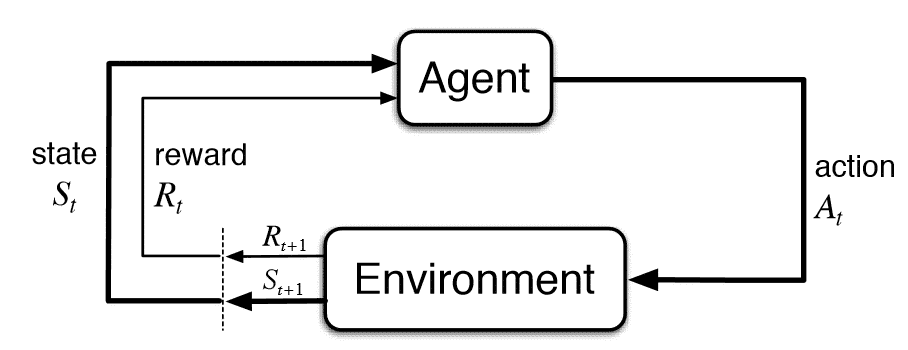
\includegraphics[height=4cm]{img/reinforcement_learning_cycle}
% 	\caption{Reinforcement learning cycle}
% 	\label{fig:reinforcement_learning_cycle}
% \end{figure}


\subsubsection{Neural networks}
\label{sub:neural_networks}

The origins of the term \textit{\gls{nn}} lie in the attempt to find mathematical representations of information processing in biological systems such as the human brain where the sheets of tissue may be understood as vectors of neurons. While assuming biological realism in pattern recognition is impractical and imposes too many unnecessary constraints, \gls{nn}s have proven to be capable of solving complex problems. The main reason for this is being able to get rid of the task of feature selection. Before the rise of \gls{nn}s, scientists and researchers had to complete the laborious task of coming up with good features to solve learning problems. Their structure enables the learning of useful representations of the input data by creating complex data representations through the combination of simpler ones. The most simple and also most successful model of this type is known as the (three layered) \textbf{\gls{mlp}} (in the following simply denoted as \gls{nn}), which will now shortly be presented. Later on (subsection~\ref{sub:neural_language_models}), more complex neural network architectures will be presented especially under the aspect of their aptitude for \gls{nlp}tasks.

A typical linear model for regression or classification is based on linear combinations of fixed nonlinear basis functions $ \phi_j (\pmb{x}) $ and takes on the form
\begin{equation}
	\label{eq:lin_comb_of_nonlinear_basis_func}
	y(\pmb{x}, \pmb{w}) = f \left( \sum_{j=1}^{M} w_j \phi_j (\pmb{x}) \right)
\end{equation}
where $ f(\cdot) $ is a nonlinear activation function. How \gls{nn}s extend this model is by making the basis functions $ \phi_j(\pmb{x}) $ depend on the parameters and then allow these parameters to be adjusted, along with the coefficients $  \{w_j\} $ during training. This gives us a basic \gls{nn} that can be described as a series of functional transformations. First, $ M $ linear combinations of the input variables $ x_1, \dots, x_D $ in the form
\begin{equation}
	a_j = \sum_{i=1}^{D} w_{ji}^{(1)} x_i + w_{j0}^{(1)}
\end{equation}
need to be constructed where $ j = 1, \dots, M $ with $ M $ being the number of hidden neurons, $ D $ denotes the input dimension and the superscript $ (1) $ indicates that the corresponding parameters are in the first `layer' of the network. The model parameters $ w_{ji}^{(1)} $ are called \textit{weights} and the parameters $ w_{j0} $ are called \textit{biases}. The term $ a_j $ is known as an \textit{activation}. Each activation is then transformed using a differentiable, nonlinear \textit{activation function} $ h (\cdot) $ to give the final output of a neuron:
\begin{equation}
	z_j = h(a_j)
\end{equation}
These quantities are called the \textit{hidden units}. The introduction of non-linearity into the network through these activation functions is a key factor in the success of \gls{nn}s as only using linear activation functions would allow for a creation of an equivalent network without hidden units. This is due to the fact that the composition of successive linear transformations is itself a linear transformation~\footnote{\url{http://www.math.lsa.umich.edu/~kesmith/217worksheet2-3ALT1.pdf}}. As for the implementation of these activation functions there exist different variants that will be listed and explained in the paragraph '\nameref{par:activation_function}'. Following equation~\ref{eq:lin_comb_of_nonlinear_basis_func}, these values are again linearly combined to give \textit{output unit activations}
\begin{equation}
	\label{eq:output_unit_activation}
	a_k = \sum_{j=1}^{M} w_{kj}^{(2)} z_j + w_{k0}^{(2)}
\end{equation}
where $ k = 1, \dots, K $ and $ K $ is the total number of outputs. Equation~\ref{eq:output_unit_activation} represents the second layer of the network. Finally, the output unit activations are transformed using an appropriate activation function to give a set of network ouputs $ y_k $. \\
Now, we can combine these various stages to give the overall network function that takes the form
\begin{equation}
	y_k(\pmb{x}, \pmb{w}) = f \left( \sum_{j=1}^{M} w_{kj}^{(2)} h \left( \frac{1}{2} \right) + w_{k0}^{(2)} \right)
\end{equation}
Thus the neural network model is simply a nonlinear function from a set of input variables $ \{x_i\} $ to a set of output variables $ \{y_k\} $ controlled by a vector $ w $ of adjustable parameters.

Figure~\ref{fig:neural_network_architecture} shows the main components of the \gls{mlp}. The input, hidden, and output variables, or units, are represented by nodes, and the weight parameters, or simply \textit{weights}, are represented by links between the nodes. Additionally, bias parameters, or simply \textit{biases}, are denoted by links coming from additional input and hidden variables $ x_0 $ and $ z_0 $. The arrows demonstrate the direction of information flow through the network during forward propagation.
\begin{figure}
	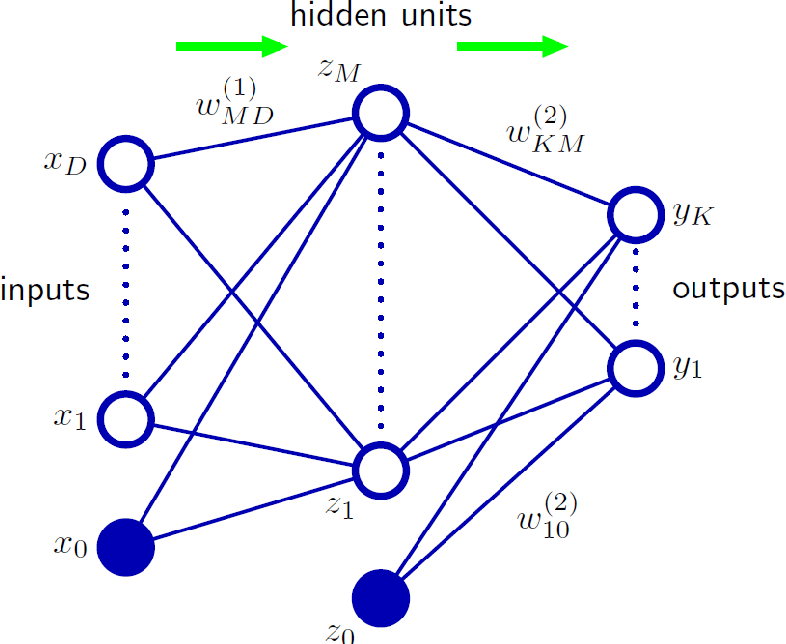
\includegraphics[height=8cm]{img/neural_network_structure}
	\caption{Neural network architecture}
	\label{fig:neural_network_architecture}
\end{figure}

\paragraph{Training process}\label{par:training_process}
The actual tuning of the network's weights are not determined exactly but are usually initialized randomly and iteratively optimized using training data via \textbf{forward propagation}. As this falls into the category of supervised learning, the desired outputs for the training inputs are known and thus a \textbf{cost} or \textbf{loss} function can be used to assess the discrepancy between prediction and ground truth. The calculated error can be used to determine the necessary updates on the weights to improve the predictions in a process called \textbf{backpropagation}. These steps will now be explained individually and in detail.

\paragraph{Activation function}\label{par:activation_function}
In analogy to our biological neurons, artificial neurons can fire a signal depending on the provided input to communicate with the following neurons (or in biology: with the neurotransmitters through electrical impulses). The decision whether a neuron fires or not lies with the activation function. After a single neuron calculates a weighted sum of its input and adds a bias to it, the value of the calculation can be anything from $ -\infty $ to $ +\infty $. As the neuron does not know the bounds of the value it uses an activation function to determine whether it should fire a signal or not.
The easiest option would be to just implement a threshold that fires if $ y > 0 $ and else does not. This, however, poses a problem when dealing with for example multi-classification. In a setting where we have 10 classes and have 2 neurons firing we can not safely say which class the model is more confident on. It would be more helpful to have instead an output of `60\%' or `90\%' activation. A linear function would also not be suited, because of the aforementioned possibility that many linear layers can be replaced by a single layer. That is why most \gls{nn}s nowadays use well-known and established activation functions in their architectures. One of the oldest but still widely used activations is the \textbf{sigmoid function} (in the form of the logistic function)
\begin{equation}
	S(x) = \frac{1}{1+e^{-x}} = \frac {e^{x}}{e^{x}+1}
\end{equation}
The sigmoid function is nonlinear and has no binary activations. Furthermore, it has a smooth gradient which means that the output does not jump in big value ranges. Sigmoids are especially suited for classification tasks, as they tend to bring activations to either `side' of the curve allowing for clear distinctions on prediction. Nonetheless, sigmoids also have a downside: Towards the edges of the domain, the slope on the $ y $-values increases (decreases) less and less which in turn also makes the gradient smaller. This poses a problem as the gradient amongst other things dictates the learning progress of the neural network - and a non-existent gradient also means that there is no learning progress (this problem is typically referred to as \textit{vanishing gradient}). Another frequently mentioned activation function is the \textbf{hyperbolic tangent}
\begin{equation}
	\tanh(x) = \frac{\sinh(x)}{\cosh(x)} = \frac{e^{x}-e^{-x}}{e^{x}+e^{-x}} = \frac{e^{2x}-1}{e^{2x}+1}
\end{equation}
which is basically a scaled sigmoid function. The $ tanh $ function was introduced in order to provide a stronger gradient than sigmoid (for steeper derivatives). Whether sigmoid or tanh activation functions should be chosen depends on the nature of the problem. The sigmoid activation function saturates at zero and one while tanh saturates at plus and minus one. So if the activity in the network during training is close to zero then the gradient for the sigmoid activation function may go to zero. However, the activation function that has had by far the most impact in the world of \gls{ml} and especially deep learning is the \textbf{\gls{relu}}
\begin{equation}
	f(x) = x^{+} = \max(0,x)
\end{equation}
simply because of its non-saturation gradient, which greatly accelerates the convergence of stochastic gradient descent compared to the other two functions~\footcite{10.1145/3065386}. Another useful property of the \gls{relu} function is that it does not need any expensive operations (e.g. exponentials) to be computed, but can simply be implemented by thresholding a matrix of activations at zero.
\begin{figure}
	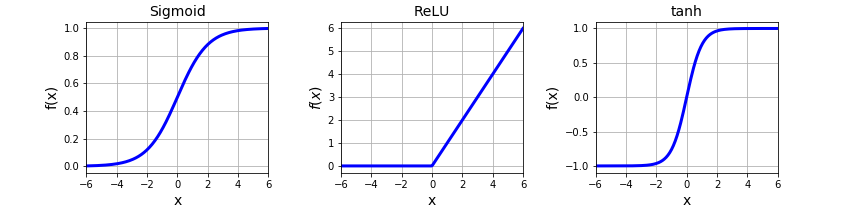
\includegraphics[height=4cm]{img/activation_functions}
	\caption{Different activation functions}
	\label{fig:different_activation_functions}
\end{figure}

\paragraph{Cost function}\label{par:cost_function}
For a neural network to know how and when to update its parameters it needs to know what the underlying optimization problem is that it is facing. This is posed by the so-called \textit{cost function}, or \textit{loss function}, which compares the prediction of the model with the desired value and returns a metric of distance. The gradient at the given input values determines the updates that the neural network will perform on its weights and biases. In the following, two of the most prominent loss functions will be presented and explained. Here, $ y $ denotes the true solution and $ \widetilde{y} $ denotes the prediction as a function $ h $ with parameters $ \theta $ of the input $ x $ of the model. The general equation of a cost function represents the sum of the errors multiplied across the whole batch:
\begin{equation}
	J(\theta) = \frac{1}{\alpha} \sum_{i=1}^{n} \text{C} (h_{\theta} (y^{(i)}), \widetilde{y}^{(i)})
\end{equation}
A simple implementation of the cost function is the \textbf{\gls{mse}} loss, which has analogies to many fields such as mechanical engineering~\footnote{\url{https://projecteuclid.org/download/pdf_1/euclid.bbms/1203692451}}. Here, the square of the difference between prediction and truth is squared, summed up and then divided by the length of the batch.
\begin{equation}
	\frac{1}{N} \sum_{i=1}^{N} \left( y_i - \widetilde{y_i} \right)^2
\end{equation}
One of the standard functions when it comes to classification is the cross-entropy loss function that calculates on step $ t $ the cross-entropy between predicted probability distribution $ \hat{y}^{(t)} $, and the truth $ y^{(t)} $
\begin{equation}
	J^{(t)}(\theta) = \text{CE}(\pmb{y}^{(t)}, \hat{\pmb{y}}^{(t)}) = - \sum_{w \in V} \pmb{y}_w^{(t)} \ \text{log} \ \hat{\pmb{y}}_w^{(t)} = - \text{log} \ \hat{\pmb{y}}_{\pmb{x}_{t+1}}^{(t)}
\end{equation}
Cross entropy relies on probabilities and not just boolean values for class membership, therefore, it allows more precise performance evaluation. Abstractly, cross entropy between two probability distributions can be interpreted as the expected message-length per datum when a wrong distribution $ q $ is assumed while the data actually follows a distribution $ p $.

\paragraph{Backpropagation}\label{par:backprop}
The process of calculating the activations at each hidden layer and the output layers as well as the resulting loss function is known as \textbf{forward propagation}. Now, to actually update the parameters of the neural network the \textit{contribution} of each parameter to the loss (gradient) needs to be computed and each parameter needs to be updated with gradient descent - this process is called \textbf{backpropagation}. The concept of gradient descent can be illustrated in a two-dimensional setting by plotting the `landscape' of the loss function which one is trying to minimize - here the initial value can be seen as the start position of a `ball' that then starts to roll down until it reaches the bottom, or mathematically: the local minimum (figure~\ref{fig:gradient_descent}). The idea of backpropagation was introduced in the 1970s by Finnish master student Seppo Linnainmaa~\footcite{linnainmaa1970representation}. Here, instead of naively calculating the gradient of each layer separately the partial computations of the gradient for each layer are reused in the computation of the gradient for the previous layer. The backpropagation algorithm is dependent on the following 5 equations:

The partial derivatives of the cost function are calculated by
\begin{equation}
	\label{eq:backprop_one}
	\frac{\delta J}{\delta w_{ij}^{k}} = \delta_j^k o_i^{k-1}
\end{equation}
where for each $ \delta_j^k $ is calculated on the final layer's loss term
\begin{equation}
	\label{eq:backprop_two}
	\delta_1^m = g'_o (a_1^m)(\hat{y}_d - y_d)
\end{equation}
and on the hidden layers' loss terms
\begin{equation}
	\label{eq:backprop_three}
	\delta_j^k = g'(a_j^k) \sum_{l=1}^{r^{k+1}} w_{jl}^{k+1} \delta_l^{k+1}
\end{equation}
Combination of the partial derivatives for each input-output pair are takes places like so
\begin{equation}
	\label{eq:backprop_four}
	\frac{\delta J(X, \theta)}{\delta w_{ij}^k} = \frac{1}{N} \sum_{d=1}^{N} \frac{\delta}{\delta w_{ij}^{k}} \left( \frac{1}{2} (\pmb{\hat{y}_d} - \pmb{y_d})^2 \right) = \frac{1}{N} \sum_{d=1}^{N} \frac{\delta J_d}{\delta w_{ij}^k}
\end{equation}
As for updating the weights, one uses
\begin{equation}
	\label{eq:backprop_five}
	\Delta w_{ij}^{k} = - \alpha \frac{\delta J(X, \theta)}{\delta w_{ij}^{k}}
\end{equation}
In the following the simplest form of backpropagation with simple \textit{gradient descent} will be presented.
\begin{enumerate}
	\item Firstly, the forward propagation for each input-output pair $ \pmb{x_d}, \pmb{y_d} $ has to be computed. The results $ \pmb{\hat{y}_d} $, $ \pmb{a_j^k} $ and $ o_j^k $ for each node $ j $ are then stored in layer $ k $ by proceeding from input layer $ 0 $ to the output layer $ m $.
	\item Secondly, the backward phase for each input-output pair $ \pmb{x_d}, \pmb{y_d} $ is calculated and the results $ \frac{\partial J_d}{\partial w_{ij}^{k}} $ for each weight $ w_{ij}^{k} $ connecting node $ i $ in layer $ k - 1 $ to node $ j $ in the next layer are stored starting now on the last layer $ m $ and continuing until layer $ 1 $. This step can be further split up into 3 sub-steps:
	\begin{enumerate}
		\item The term $ \delta_1^m $ is calculated by using equation~\ref{eq:backprop_two}.
		\item The calculated loss terms for the hidden layers $ \delta_j^k $ are backpropagated starting on layer $ k = m - 1 $ through repetitive usage of equation~\ref{eq:backprop_three}.
		\item Now the partial derivatives of individual loss $ J_d $ \gls{wrt} $ w_{ij}^k $ can be evaluated by using equation~\ref{eq:backprop_one}.
	\end{enumerate}
	\item Now, the entirety of the gradient $ \frac{\delta J(X, \theta)}{\delta w_{ij}^k} $ over the entire set of input-output pairs can be calculated by combining the individual input-output pair gradients in equation~\ref{eq:backprop_four}.
	\item The \textbf{learning rate} $ \alpha $ is used in the final formula to update the weights of the network by subtracting the total gradient $ \frac{\delta J(X, \theta)}{\delta w_{ij}^k} $ multiplied by $ \alpha $ (equation~\ref{eq:backprop_five}).
\end{enumerate}
\bigskip

\begin{figure}
	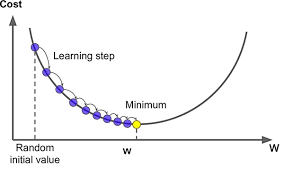
\includegraphics[height=4cm]{img/gradient_descent}
	\caption{Gradient descent on a convex quadratic function}
	\label{fig:gradient_descent}
\end{figure}

There are different variations of the gradient descent optimization, namely batch, stochastic and mini-batch, which will shortly be presented. Each variant differs in how much data is used to compute the gradient of the loss function - which one is best suited depends on the problem. These variations fundamentally are a trade-off between speed and accuracy. \textbf{Batch gradient descent} utilizes the whole dataset, computing the loss of each data point and averaging over the entire set. This takes up a lot of computation, therefore batch gradient descent is considered to be slow. Also using each datapoint many times can cause the algorithm to overfit on the training data. Batch gradient descent works best for functions with very little local minima, as it can easily get stuck in one. In contrast, \textbf{\gls{sgd}} computes the loss and makes the update on a single sample rather than the entire set. This speeds up each gradient step linearly with the size of the data set. Due to noise in the data it can happen though, that the gradient step is performed in the opposite direction of the optimum. \gls{sgd} works best if the function has a lot of local minima since the noise performing the gradient descent on a single data point oftentimes moves the model out of local minimum to maybe a better one. \textbf{Mini-Batch} uses a random subset of the entire dataset and computes the gradient of the loss on that subset. This is a combination of the other two methods so it can reduce the problems they are facing. It takes way less computation performing one step while reducing the noisiness of \gls{sgd}. Choosing the mini-batch size depends on the problem. If possible it should be small enough to still avoid local minima, while being big enough to converge to the global minimum.



\subsubsection{Recent developments}
\label{sub:recent_developments}

Here I write about recent developments.

\subsubsection{Practical applications}
\label{sub:practical_applications}

Here I write about practical applications.

\subsection{History of language modeling}
\label{sec:history_of_language_modeling}

Natural language processing (NLP) is “an area of research and application that explores how computers can be used to
understand and manipulate natural language text or speech to do useful things”~\footcite{doi:10.1002/aris.1440370103}.
The applications of NLP such as speech recognition, sentiment analysis,
question answering and others are numerous~\footcite{DBLP:journals/corr/GattK17}.
Moreover, these applications are already being heavily used by industry and
consumers alike e.g. in the forms of digital voice assistants, sentiment analysis for recommender systems
and browser search bars~\footcite{8012330,10.1145/3064663.3064672,GoogleSearch}. The subcomponent of NLP
needed when it comes to tasks like machine translation, predictive typing or summarization that involve either
generating text or estimating the probability of text is called language modeling. The following notation mostly
follows the one from the CS224 Stanford Natural Language Processing with Deep Learning lecutre by Chris Manning~\footnote{\url{https://web.stanford.edu/class/cs224n/index.html}}. The following chapters will cover word representation (ch.~\ref{sub:word_representation}) as the foundation for language models, followed by a brief explanation of the basics of language models (ch.~\ref{sub:foundations_of_language_modeling}) and will end with the most common and most used language model types and architectures (ch.~\ref{sub:n_gram_models} - ch.~\ref{sub:neural_language_models}).

\subsubsection{Word representation}
\label{sub:word_representation}

The starting point for most NLP related tasks lies within the preprocessing of the textual input data. These must first be converted into a semantically meaningful numerical representation to allow for effective computation. The simplest way to represent a word numerically is by treating words as \textit{one-hot} vectors. Using this format, one word is encoded into an $ n $-dimensional vector of numbers where $ n $ is the vocabulary size and each entry takes on the value $ 0 $ except for the one that corresponds to the indexed word which takes on the value $ 1 $. This process generates very sparse feature vectors for each input word, which is no problem for simple classification tasks, but is unsuitable for larger problems as the dimension size increases for each word added to the vocabulary. Another issue of one-hot vectors is the fact that these representations hold no notion of similarity: If we take a look at the representations for the words “plane“ and “airplane“ we would get two vectors that are orthogonal, just as any two vectors in the whole vocabulary. This poses a problem as every word's similarity to other words is the same and we can not encapsulate the meaning of the word. Yoav Goldberg writes in his primer on neural networks for language processing that one-hot vectors should only be considered for problems where the model has only a small amount of input features, the inputs do not have to share model parameters and where there is a lot of data to learn from~\footcite{DBLP:journals/corr/Goldberg15c}.

Otherwise, the currently dominant approach in the field is to use word embeddings as feature vectors. Word embeddings follow the so called “distributional semantics“, which state that a word's meaning is given by the words that tend to occur in a similar context. This idea of context-dependent nature of meaning was first introduced by english linguist J.R. Firth~\footnote{\url{https://web.stanford.edu/class/linguist236/materials/ling236-handout-05-09-vsm.pdf}} with the famous quote:

\begin{quote}
  You shall know a word by the company it keeps.
\end{quote}

Following this idea we represent each word by a distribution of weights across many dimensions. Now, instead of having a one-to-one mapping between an element in the vector and a word, the representation of a word is spread across all of the entries in the vector, and each element in the vector contributes to the definition of many words. Having this new form of word vectors allows us to capture meaningful semantic and syntactic regularities between words in an expressive way. A simple way to illustrate this is depicted in figure~\ref{fig:word2vec_king_queen_composition}. \\
Here, our word vectors contain the knowledge that the difference between a “king“ and a “queen“ primarily lies within the gender of a person. Thus, if we subtract the word vector of “man“ from “king“ and we add the word vector of “woman“ we get a word vector that is very similar to the one of “queen“.

\begin{figure}[h]
  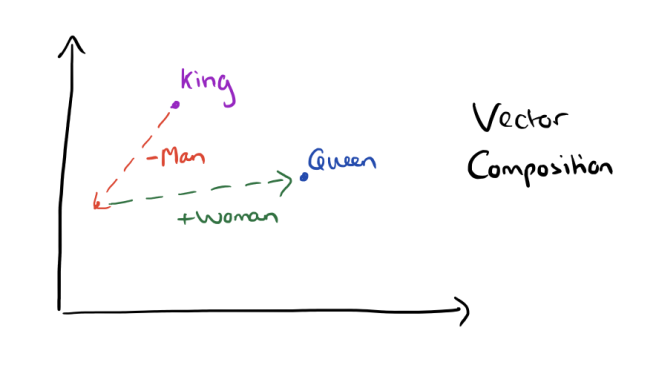
\includegraphics[height=5cm]{img/word2vec-king-queen-composition}
  \caption{Word2vec king queen composition}
\label{fig:word2vec_king_queen_composition}
\end{figure}

The most famous realization of these embeddings was introduced by the researchers of Google around Tomas Mikolov in their paper “Distributed Representations of Words and Phrases and their Compositionality“~\footcite{DBLP:journals/corr/MikolovSCCD13}. Hereafter, their proposed approach, Word2Vec, along with their used notation will briefly be presented, as its core ideas are found throughout other popular word embedding frameworks as well. \\
Given a sequence of training words $ w_1, w_2, \dots, w_T $, the objective (paragraph~\ref{par:cost_function}) is to minimize the average negative log likelihood
\begin{equation}
	\label{eqn:skip_gram_objective_function}
	J(\theta) = - \frac{1}{T} \sum_{t=1}^{T} \sum_{\substack{-m \leq j \leq m \\ j \neq 0}} \text{log} \ P(w_{t+j} | w_t; \theta)
\end{equation}
where $ m $ is the fixed window size containing the context words around the center word $ w_j $. Enlarging this window size results in more training examples and can lead to a higher accuracy, at the expense of training time. In order to compute the term $ P(w_{t+j} | w_t; \theta) $ a regular softmax function (ch 3.3.3 [HARDCODED, ref to softmax function]) can be applied
\begin{equation}
	\label{eqn:skip_gram_conditional_probability}
	P(o | c) = \frac{\text{exp} \ (u_{o}^{T} v_{c})}{\sum_{w \in V} \text{exp} \ (u_{w}^{T} v_c)}
\end{equation}
where we use two vectors per word $ w $: $ v_w $ when $ w $ is a center word and $ u_w $ when $ w $ is a context word. Optimizing the objective function results in high-quality distributed vector representations. It should be noted that for computational efficiency modified versions of these functions such as negative sampling or hierarchical softmax are used, as the presented ones do not scale well.

Even though word2vec embeddings are a powerful representation they do face certain limitations, which is why \textit{Stanford University}~\footnote{\url{https://www.stanford.edu}} took it upon itself to create an improved variant called GloVe~\footcite{pennington-etal-2014-glove}. While word2vec ignores that some context words appear more ofthen than others, GloVe stresses the importance of frequencies of co-occurrences and that these should not be “wasted“ as additional training examples. Therefore, GloVe builds word embeddings in a way that a combination of word vectors relates directly to the probability of these words' co-occurrence in the corpus. \\
Another alternative to word2vec is \textit{fasttext} by Facebook, which generates word vectors that generalize better, need less training data and can be trained “on more than one billion words in less than ten minutes using a standard multicore CPU, and classify half a million sentences among 312K classes in less than a minute“ according to the authors~\footcite{DBLP:journals/corr/JoulinGBM16}. FastText also takes word parts into account, i.e. FastText not only stays on a word level of depth but also goes into the character level.


\subsubsection{Foundations of language modeling}
\label{sub:foundations_of_language_modeling}

As the necessary preprocessing has been dealt with, we can now get to the actual task of language modeling, which is the task of predicting “what word comes next“. More formally, this means: Given a sequence of words $ x^{(1)}, x^{(2)}, \dots, x^{(t)} $, compute the probability of the next word $ x^{(t+1)} $:
\begin{equation}
    P(x^{(t+1)} | x^{(t)}, \dots, x^{(1)})
\end{equation}
where $ x^{(t+1)} $ can be any word in the vocabulary $ V = \{w_1, \dots, w_{|V|}\} $.  \\
Having a system that does so allows us to assign a probability to a text excerpt of length $ T $:
\begin{align}
    \begin{split}
    P(x^{(1)}, \dots, x^{(T)}) &= P(x^{(1)}) \times P(x^{(2)} | x^{(1)}) \times \cdots \times P(x^{(T)} | x^{(T-1)}, \dots, x^{(1)}) \\
    &= \prod_{t=1}^{T} P(x^{(t)} | x^{(t-1)}, \dots, x^{(1)})
    \end{split}
\end{align}
Developing and improving language models is a task central to language understanding by which we can measure how well machine learning systems actually comprehend natural language. This is demonstrated by the fact that “often (although not always), training better language models improves the underlying metrics of the downstream task (such as word error rate for speech recognition, or BLEU score for translation), which makes the task of training better LMs valuable by itself”~\footcite{DBLP:journals/corr/JozefowiczVSSW16}. \\
Since the first significant language model was proposed back in 1980~\footcite{880083}, language models and their architectures have gone through many changes. Especially the rise of deep learning and new network models such as recurrent neural networks (RNNs) or transformers have fueled language modeling research in the past few years.


\subsubsection{N-Gram models}
\label{sub:n_gram_models}

One solution in dealing with the problem of predicting a word after a sequence of $ (n - 1) $
words in the form of a Markov model, i.e. the probability of each event depends only on the state
attained through the previous event, is called an n-gram model. An “n-gram” hereby denotes a chunk 
of n consecutive words. The core idea is that the probability of a word $ w_i $ occurring in the 
$ i^{th} $ instance after a sequence of $ (i - 1) $ preceding words can be approximated by observing 
only the preceding context of $ (n - 1) $ words.

Following this insight we can compute the probability of all n-grams in a corpus of text by simply counting their occurrences.
Doing so allows us to calculate the conditional probabilities like so:
\begin{align}
    \begin{split}
        P(x^{(t+1)} | x^{(t)}, \dots, x^{(1)}) &= P(x^{(t+1)} | x^{(t)}, \dots, x^{(t - 2 + 2)}) \\ \\
        &= \frac{P(x^{(t+1)}, x^{(t)}, \dots, x^{(t - 2 + 2)})}{P(x^{(t)}, \dots, x^{(t - 2 + 2)})} \\ \\
        &\approx \frac{\text{count}(x^{(t+1)}, x^{(t)}, \dots, x^{(t - n + 2)})}{\text{count}(x^{(t)}, \dots, x^{(t - n + 2)})}
    \end{split}
\end{align}
N-gram models where $ n = 1 $, $ n = 2 $ and $ n = 3 $ are called unigram, bigram and trigram, respectively. The parameter $ n $ typically does not get bigger than $ 5 $. Having the conditional probabilites new text can be generated by conditioning on the provided input. After getting a probability distribution over the vocabulary a sampling strategy (ch. 3.3.3 [HARDCODED]) that returns a word has to be applied.

Even though n-gram models have been widely used especially due to their simplicity and scalability they do face certain limitations that have led to a decrease in their popularity. One problem that can occur is the one of unexpected n-grams: if the $ n $-gram encountered in the test setting did not appear in the corpus that the model was trained on, then the probability for the $ n^{th} $ word conditioned on the $ (n-1) $ words is $ 0 $. If an $ (n-1) $-gram is encountered in the test setting but not in the training data, then the model can not calculate the probability of any word that comes after. These two sparsity limitations can, however, partly be encountered by using smoothing and backoff techniques. The storage problem is evident, as increasing $ n $ or simply enlarging the training corpus increases the model size, which poses a significant problem for larger NLP applications. The implications of this restriction can be withdrawn from the following illustrative generated text snippet:

\begin{quote}
“today the price of gold per ton , while production of shoe lasts and shoe industry , the bank intervened just after it considered and rejected an imf demand to rebuild depleted european stocks , sept 30 end primary 76 cts a share”
\end{quote}

Because of the inability to expand the context window effectively, we remain tied to a LM that can generate grammatical but also incoherent model that can not relate predictions to history reaching further into the past. N-gram language models are still widely used in speech recognition due to their high efficiency in inference~\footcite{wang2019improving} but their limitations caused by poor generalization to unobserved n-grams and inability to capture long range dependencies led to the rise of neural language models.





\subsubsection{Neural language models}
\label{sub:neural_language_models}

\paragraph{Neural network}
This is some text.

\paragraph{Recurrent neural networks}
This is some text.

\paragraph{Convolutional neural networks}
This is some text.

\paragraph{Attention and transformers}
This is some text.
